\section{Seguimiento de carriles}

\begin{frame}\frametitle{Modelo cinemático}
  Considere la base móvil de la figura:
  \begin{figure}
    \centering
    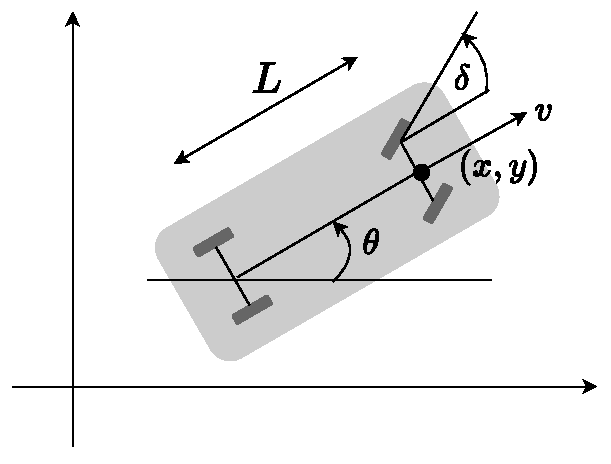
\includegraphics[width=0.3\textwidth]{Figuras/Ackermann.pdf}
  \end{figure}
  con
  \begin{itemize}
  \item $(x,y,\theta)$ la configuración en el plano de movimiento, considerando como centro el centro del eje delantero (tracción delantera)
  \item $L$ la distancia entre ejes de las llantas
  \item $v$ es la velocidad lineal del vehículo considerada como señal de entrada
  \item $\delta$ es el ángulo de las llantas delanteras (volante) también considerada como señal de control
  \end{itemize}
  El objetivo es determinar $v$ y $\delta$ de modo que le vehículo tenga determinado comportamiento.
\end{frame}

\begin{frame}\frametitle{Seguimiento de carriles}
  El seguimiento de carriles se puede hacer con base en las líneas detectadas. Considere la figura:
  \begin{figure}
    \centering
    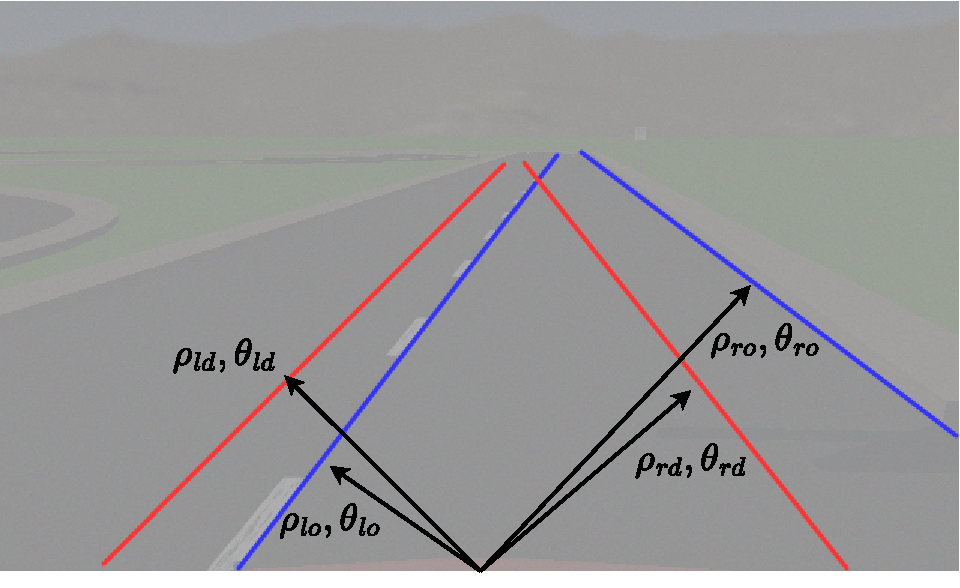
\includegraphics[width=0.5\textwidth]{Figuras/LineErrors.pdf}
  \end{figure}
  \begin{itemize}
  \item Las líneas azules son los bordes observados y las líneas rojas son las líneas que se deberían observar si el auto estuviera bien centrado y alineado en el carril.
  \item La diferencia entre los parámetros observados $(\rho_o,\theta_o)$ y los parámetros deseados $(\rho_d, \theta_d)$ se puede utilizar para calcular las señales $v,\delta$
  \end{itemize}
\end{frame}

\begin{frame}\frametitle{Seguimiento de carriles}
  \begin{itemize}
  \item El sterring $\delta$ se puede calcular con un control proporcional al error entre líneas deseadas y líneas observadas
  \item La velocidad lineal se puede calcular para que sea más pequeña cuando el auto esté girando
  \end{itemize}
  \begin{eqnarray*}
    \delta &=& K_\rho e_\rho + K_\theta e_\theta\\
    v &=& v_{max}(1 - k_\delta |\delta|)
  \end{eqnarray*}
  con
  \[
    e_\rho = \left\{ \begin{array}{lcl}
      \frac{1}{2}(\rho_{lo} - \rho_{ld} + \rho_{rd} - \rho_{ro}) & \textrm{si} & \rho_{lo}\neq 0\; , \; \rho_{ro} \neq 0\\
      (\rho_{lo} - \rho_{ld}) & \textrm{si} & \rho_{lo}\neq 0\\
      (\rho_{rd} - \rho_{ro}) & \textrm{en otro caso} & 
      \end{array}
    \right.\]
  \[
    e_\theta = \left\{ \begin{array}{lcl}
      \frac{1}{2}(\theta_{lo} - \theta_{ld} + \theta_{rd} - \theta_{ro}) & \textrm{si} & \theta_{lo}\neq 0\; , \; \theta_{ro} \neq 0\\
      (\theta_{lo} - \theta_{ld}) & \textrm{si} & \theta_{lo}\neq 0\\
      (\theta_{rd} - \theta_{ro}) & \textrm{en otro caso} & 
      \end{array}
    \right.\]
  y $K_\rho > 0$, $K_\theta > 0$, $k_\delta > 0$
\end{frame}

\begin{frame}[containsverbatim]\frametitle{Ejercicio 06 - Seguimiento de carriles}
  \begin{enumerate}
  \item Abra el archivo fuente del ejercicio 06 y agregue el siguiente código en la línea 27:
    \begin{lstlisting}[language=Python, firstnumber=27]
if rho_l != 0 and rho_r != 0:
    error_rho   = (rho_l   - goal_rho_l   + goal_rho_r   - rho_r)/2
    error_theta = (theta_l - goal_theta_l + goal_theta_r - theta_r)/2
elif rho_l != 0:
    error_rho   = rho_l   - goal_rho_l  
    error_theta = theta_l - goal_theta_l
else:
    error_rho   = goal_rho_r   - rho_r  
    error_theta = goal_theta_r - theta_r
steering = k_rho*error_rho + k_theta*error_theta
speed = max_speed*(1 - k_delta*abs(steering))
    \end{lstlisting}
  \item Abra una terminal y ejecute la simulación con el comando:
    \begin{lstlisting}[language=bash,numbers=none]
roslaunch eir2024 navigation_no_obstacles.launch
    \end{lstlisting}
  \item En otra terminal ejecute el ejercicio 05 (detección de carriles) con el comando:
    \begin{lstlisting}[language=bash,numbers=none]
rosrun eir2024 exercise05.py 
    \end{lstlisting}
  \end{enumerate}
\end{frame}

\begin{frame}[containsverbatim]\frametitle{Ejercicio 06 - Seguimiento de carriles}
  \begin{enumerate}
    \setcounter{enumi}{3}
  \item En otra terminal, ejecute el ejercicio 06 con el comando:
    \begin{lstlisting}[language=bash,numbers=none]
rosrun eir2024 exercise06.py _k_rho:=0.001 _k_theta:=0.01 _max_speed:=20
    \end{lstlisting}
  \item Observe el comportamiento del vehículo y sintonice las constantes $k_\rho$ y $k_\theta$.
  \item Cuando estén sintonizadas las constantes, pruebe con velocidades $v_{max}$ más altas.
  \end{enumerate}
\end{frame}